\section{Agentic Image Generation, Editing, and Restoration}
\label{sec:image-generation}

Image creation agents must control an evolving artifact whose relevant state can include composition, masks, object identity, references, edit history, degradation estimates, user preferences, and tool outputs. Section~\ref{sec:analytical-framework} identifies the analytical components used to compare these systems. This section instead organizes image-domain studies by the primary contribution that they demonstrate. Each paper is assigned one location; secondary mechanisms remain relevant for cross-cutting comparison but do not determine a second placement.

\begin{figure}[!htbp]
  \centering
  
\definecolor{avgmapblue}{HTML}{22558A}
\definecolor{avgmapgreen}{HTML}{23845D}
\ifdefined\avgmapfont\else\newcommand{\avgmapfont}{\rmfamily}\fi
\makebox[\linewidth][c]{%
\resizebox{0.98\linewidth}{!}{%
\begin{tikzpicture}[
  avg branch/.style={draw=avgmapblue!58, fill=avgmapblue!9, text=black!88, rounded corners=2.5pt, line width=0.48pt, text width=42mm, minimum height=8.8mm, align=center, inner xsep=2.2mm, inner ysep=0.9mm, outer sep=0pt, execute at begin node={\hyphenpenalty=10000\exhyphenpenalty=10000\relax}, font=\avgmapfont\fontsize{7.35}{8.35}\selectfont\bfseries},
  avg papers/.style={draw=avgmapblue!25, fill=avgmapblue!2, text=black!88, rounded corners=2.5pt, line width=0.38pt, text width=115mm, minimum height=8.8mm, align=left, inner xsep=3mm, inner ysep=0.9mm, outer sep=0pt, execute at begin node={\hyphenpenalty=10000\exhyphenpenalty=10000\relax}, font=\avgmapfont\fontsize{7.15}{8.25}\selectfont\bfseries},
  avg benchmark branch/.style={avg branch, draw=avgmapgreen!78, fill=avgmapgreen!15, text=avgmapgreen!45!black},
  avg benchmark papers/.style={avg papers, draw=avgmapgreen!72, fill=avgmapgreen!7, text=black!88},
  avg root/.style={draw=avgmapblue, fill=avgmapblue!94!black, text=white, rounded corners=2.5pt, line width=0.55pt, minimum width=9mm, minimum height=36mm, inner sep=0pt, outer sep=0pt},
  avg line/.style={draw=black!28, line width=0.45pt, line cap=round},
  avg benchmark line/.style={draw=avgmapgreen!78, line width=0.55pt, line cap=round}
]
\matrix (avgmap) [matrix of nodes, row sep=1.35mm, column sep=3mm, ampersand replacement=\&, nodes={anchor=center}] {
  \node[avg branch] (c4b1) {Feedback-Driven}; \& \node[avg papers] (c4p1) {Idea2Img~\cite{yang2024idea2img}, MuLan~\cite{li2025mulan}, CRAFT~\cite{kovalev2025craft}, FiRe~\cite{kim2026fire}, RefineEdit-Agent~\cite{avg250817435}, MIRA~\cite{avg251121087}, Agentic Retoucher~\cite{avg260102046}, EditRefiner~\cite{avg260507457}.}; \\
  \node[avg branch] (c4b2) {Planning and Tool Use}; \& \node[avg papers] (c4p2) {DiffusionAgent~\cite{qin2024diffusionagent}, GenAgent~\cite{jiang2026genagent}, Gen-Searcher~\cite{avg260328767}, MetaPoint~\cite{zhou2026metapoint}, Qwen-Image-Agent~\cite{avg260626907}, GenArtist~\cite{wang2024genartist}, AgenticIR~\cite{avg241017809}, CoSTA*~\cite{gupta2025costa}, TIR-Agent~\cite{avg260327742}, CanvasAgent~\cite{avg260705465}.}; \\
  \node[avg branch] (c4b3) {Stateful Systems}; \& \node[avg papers] (c4p3) {AutoStudio~\cite{cheng2024autostudio}, PASTA~\cite{nabati2025pasta}, StoryState~\cite{sarkar2026storystate}, Agent Banana~\cite{ye2026agentbanana}, Generation Navigator~\cite{avg260517969}, I2E~\cite{avg260103741}, MSRAMIE~\cite{avg260316967}, LogiStory~\cite{avg260328082}.}; \\
  \node[avg branch] (c4b4) {Multi-Agent Systems}; \& \node[avg papers] (c4p4) {Marmot~\cite{sun2025marmot}, T2I-Copilot~\cite{chen2025t2icopilot}, M3~\cite{avg260206166}, coDrawAgents~\cite{avg260312829}, MUSES~\cite{ding2025muses}, CCA~\cite{hang2024cca}, MAIR~\cite{avg250309403}, Talk2Image~\cite{avg250806916}, ImageEdit-R1~\cite{avg260308059}, CAMEO~\cite{pu2026cameo}.}; \\
  \node[avg branch] (c4b5) {Native and Unified Models}; \& \node[avg papers] (c4p5) {ImAgent~\cite{avg251111483}, UniReason 1.0~\cite{avg260202437}, VisionCreator~\cite{avg260302681}, VisionCreator-R1~\cite{avg260308812}, Unify-Agent~\cite{avg260329620}, Boogu-Image-0.1~\cite{avg260713125}, ToolArtist~\cite{zhao2026toolartist}.}; \\
  \node[avg branch] (c4b6) {Data, Evaluation, and Safety}; \& \node[avg papers] (c4p6) {Gen-n-Val~\cite{huang2025gennval}, GenEvolve~\cite{chen2026genevolve}, EvoIR-Agent~\cite{avg260522208}, OctoT2I~\cite{jiang2026octot2i}, COMFYCLAW~\cite{avg260701709}, VALOR~\cite{avg251111693}, OrchJail~\cite{avg260507414}, ConceptAgent~\cite{avg260518150}, RedEdit~\cite{avg260606140}.}; \\
  \node[avg benchmark branch] (c4b7) {Benchmarks}; \& \node[avg benchmark papers] (c4p7) {CIGEval~\cite{avg250407046}, EdiVal-Agent~\cite{avg250913399}, Blueprint-Bench~\cite{avg250925229}, ImagingBench~\cite{avg260707189}.}; \\
};
\coordinate (c4trunktop) at ($(c4b1.west)+(-4.6mm,0)$);
\coordinate (c4trunkbottom) at ($(c4b7.west)+(-4.6mm,0)$);
\coordinate (c4rootnw) at ($(c4b1.north west)+(-15.5mm,0)$);
\coordinate (c4rootse) at ($(c4b7.south west)+(-7.6mm,0)$);
\node[avg root, fit=(c4rootnw)(c4rootse)] (c4root) {};
\node[rotate=90, align=center, text=white, font=\avgmapfont\fontsize{7.05}{8.15}\selectfont] at (c4root.center) {{\bfseries CHAPTER 4}\\[0.55mm]{\fontsize{6.2}{7.15}\selectfont Image generation, editing, and restoration}};
\draw[avg line] (c4trunktop) -- (c4trunkbottom);
\coordinate (c4trunkmid) at ($(c4trunktop)!0.5!(c4trunkbottom)$);
\draw[avg line] (c4root.east) -- (c4trunkmid);
\draw[avg line] (c4trunktop |- c4b1.west) -- (c4b1.west);
\draw[avg line] (c4b1.east) -- (c4p1.west);
\draw[avg line] (c4trunktop |- c4b2.west) -- (c4b2.west);
\draw[avg line] (c4b2.east) -- (c4p2.west);
\draw[avg line] (c4trunktop |- c4b3.west) -- (c4b3.west);
\draw[avg line] (c4b3.east) -- (c4p3.west);
\draw[avg line] (c4trunktop |- c4b4.west) -- (c4b4.west);
\draw[avg line] (c4b4.east) -- (c4p4.west);
\draw[avg line] (c4trunktop |- c4b5.west) -- (c4b5.west);
\draw[avg line] (c4b5.east) -- (c4p5.west);
\draw[avg line] (c4trunktop |- c4b6.west) -- (c4b6.west);
\draw[avg line] (c4b6.east) -- (c4p6.west);
\draw[avg benchmark line] (c4trunktop |- c4b7.west) -- (c4b7.west);
\draw[avg benchmark line] (c4b7.east) -- (c4p7.west);
\end{tikzpicture}%
}%
}

  \caption{Representative systems and benchmarks for agentic image generation, editing, and restoration, organized according to the chapter taxonomy.}
  \label{fig:ch4-representative-systems}
\end{figure}

\subsection{Feedback-Driven Image Generation and Editing}
Feedback-driven systems observe a generated artifact, identify a deviation from the current goal, and revise a later generation or editing decision. The following subsections distinguish compositional and design refinement from image-level editing, completion, and restoration.

\subsubsection{Compositional Generation and Design Refinement}
These systems use generated images as evidence for revising compositional constraints, design intent, or local defects. Their common contribution is a feedback action that changes the current generation trajectory.

\paragraph{Improving Compositional Text-to-Image Generation with Large Vision-Language Models.}
This work uses an LVLM as both evaluator and editor for compositional text-to-image generation. The LVLM converts prompts into QA checks, uses answer accuracy as a loss weight for ReFL fine-tuning, and at inference iteratively detects mismatches and directs SAM+Blended Diffusion to correct them until fully compliant. ~\cite{wen2023compositional}

\paragraph{Idea2Img.}
 is a GPT-4V agent that iteratively refines prompts for multimodal image design without prior knowledge of the T2I model's optimal usage. Each round, GPT-4V generates candidate prompts, selects the best draft, reflects on mismatches with the user IDEA (interleaved text and images), and stores feedback in memory to guide revision. On 104 queries, iterative SDXL v1.0 wins 56.7\% (vs. 29.8\% initial, 13.5\% manual; +26.9 SDXL, +16.3 IF). Memory guides revision within runs; cross-run retention is untested.~\cite{yang2024idea2img} Figure~\ref{fig:ch4-feedback-refinement} illustrates how retained comparisons guide successive prompt revisions.

\begin{figure}[!htbp]
  \centering
  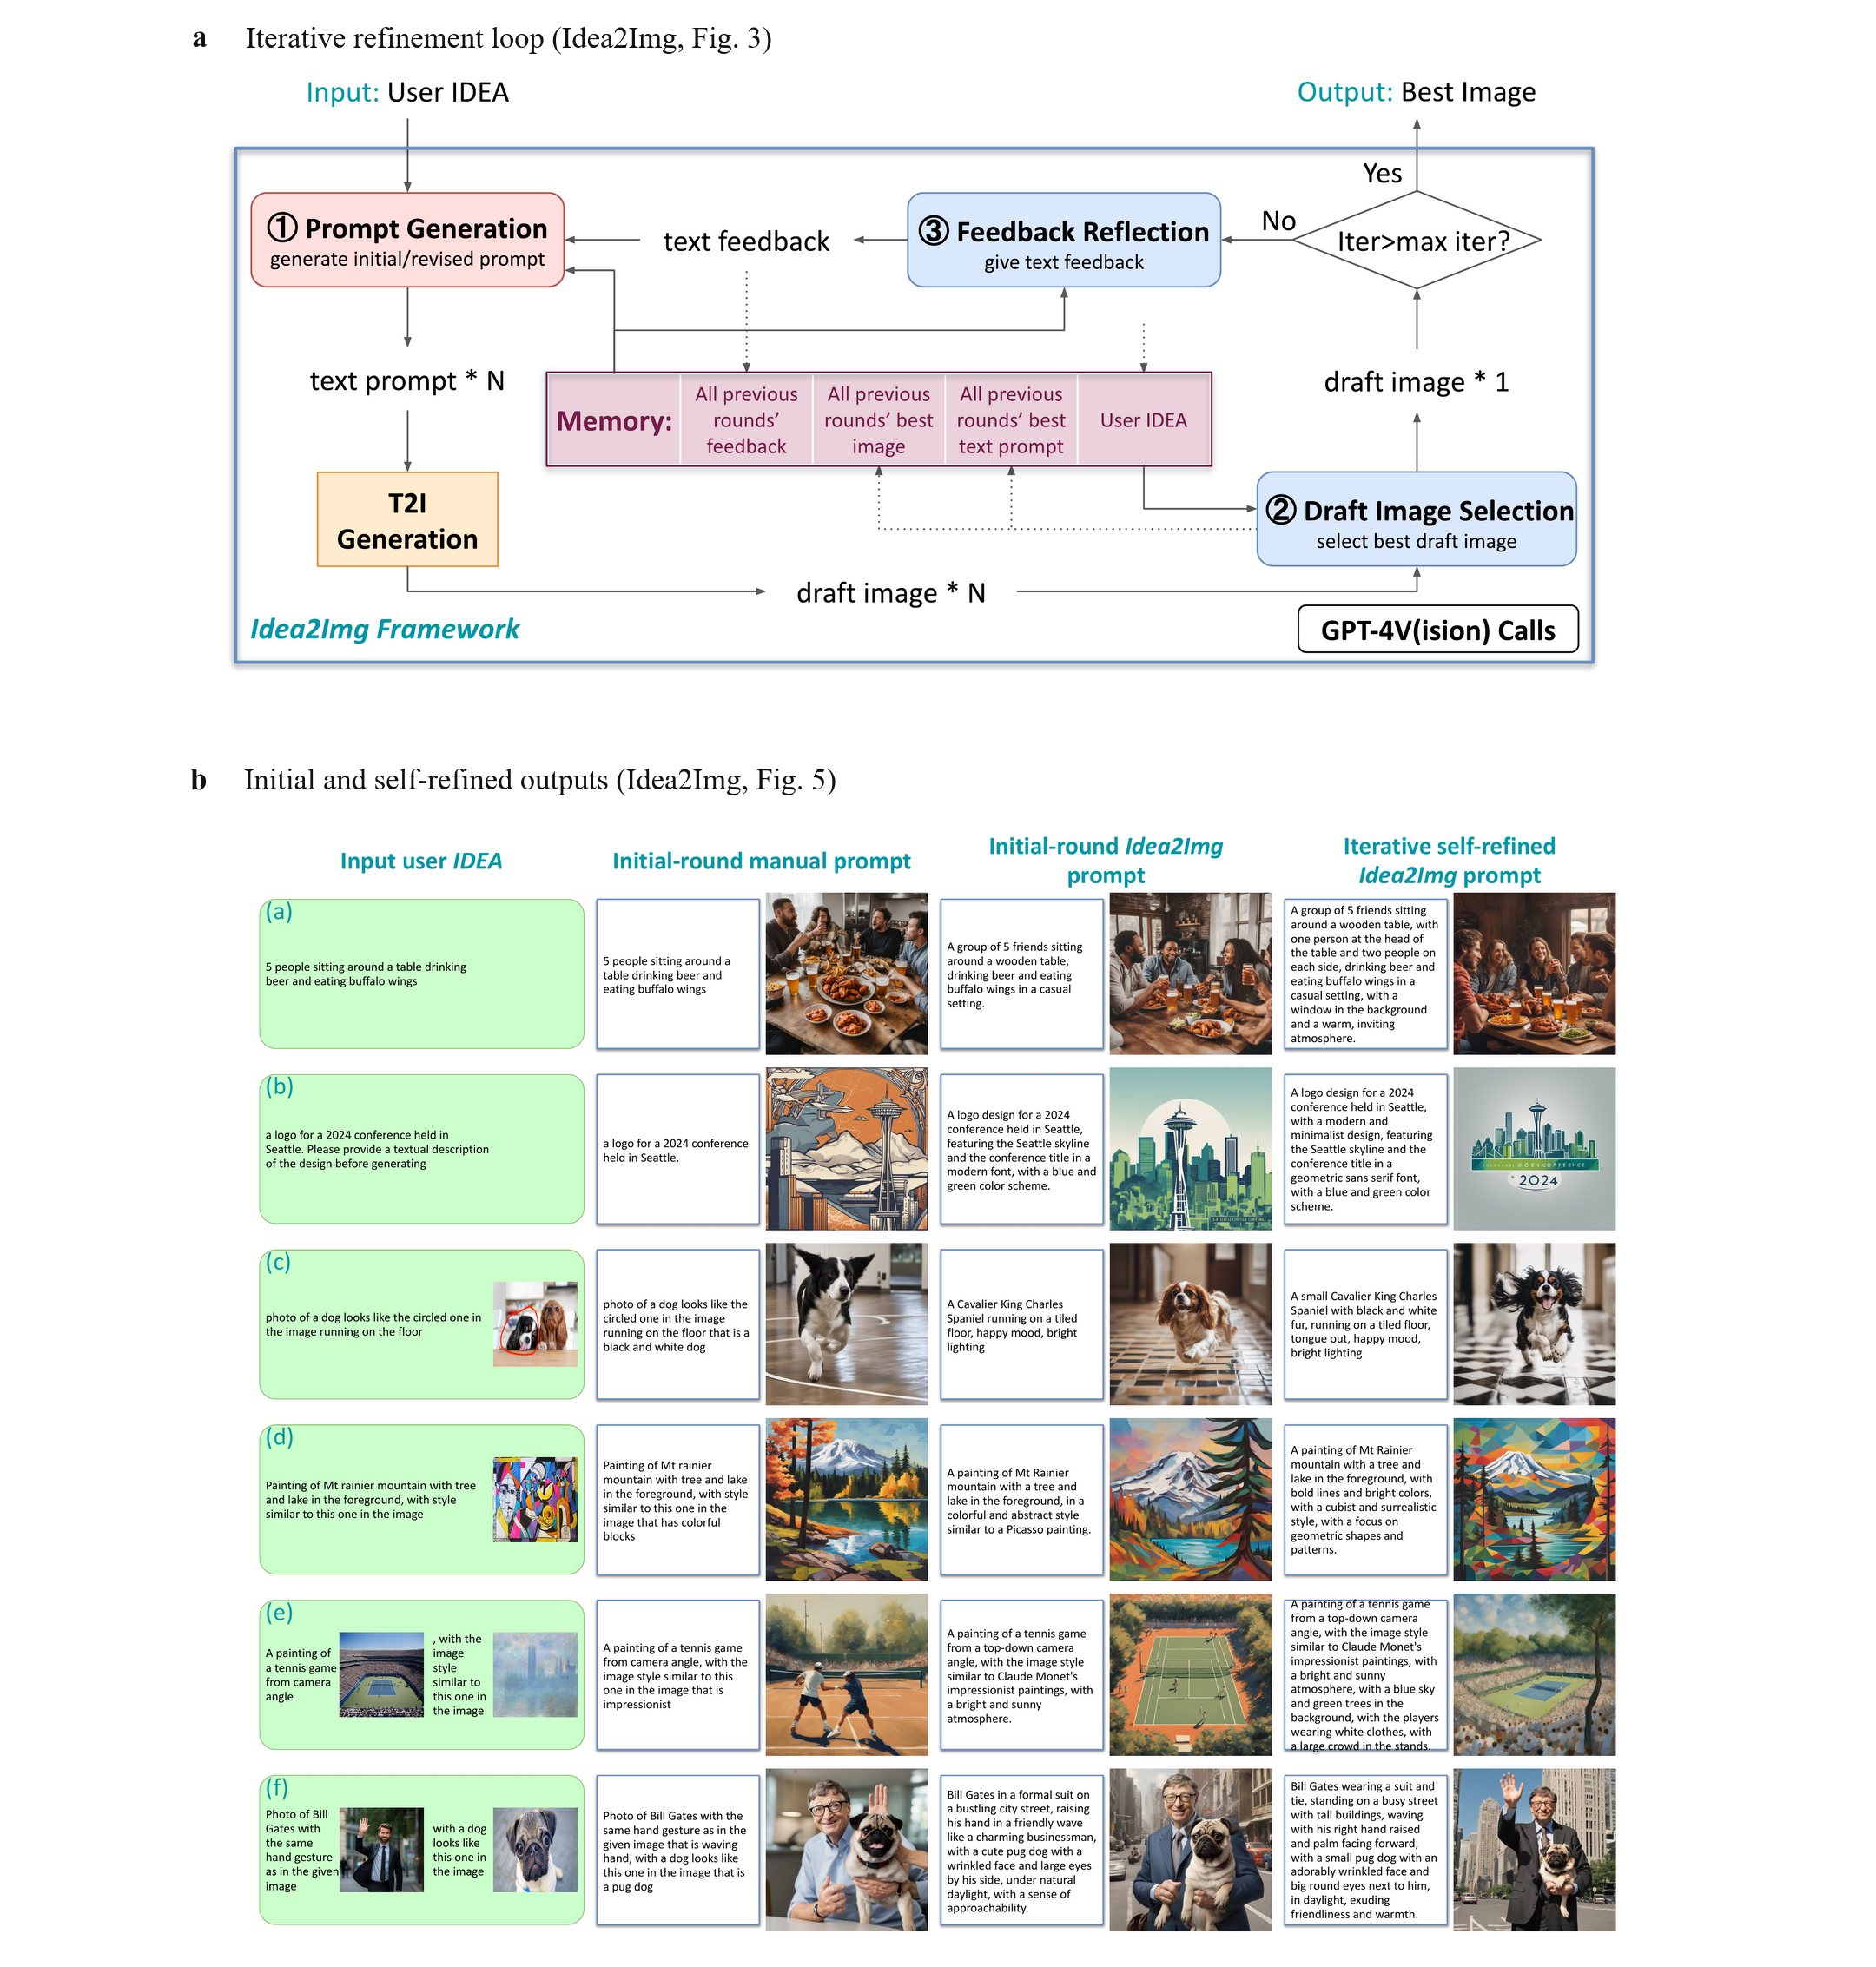
\includegraphics[width=\textwidth]{figures/ch4_feedback_driven_refinement.jpg}
  \caption{Feedback-driven image refinement. Idea2Img retains prompts, draft images, and comparative feedback within a run, then uses this memory to revise subsequent prompts; representative outputs illustrate the difference between initial and iteratively self-refined generations~\cite{yang2024idea2img}.}
  \label{fig:ch4-feedback-refinement}
\end{figure}

\paragraph{MuLan.}
 is a training-free agent that decomposes complex prompts into object-level subtasks, generating each object conditioned on prior ones via LLM-planned masks and attention guidance, with a VLM verifying each subtask and triggering regeneration on violation; users may intervene mid-process. VLM feedback proves critical.~\cite{li2025mulan}

\paragraph{VisualPrompter.}
 is a training-free prompt optimization framework that fixes semantic omissions in text-to-image generation by decomposing prompts into atomic concepts, using a VLM to identify which concepts are missing in the generated image, and revising only those units before reassembling the prompt.  ~\cite{wu2026visualprompter}

\paragraph{Maestro.}
 is a test-time agent system that automates T2I prompt refinement from underspecified user prompts. It decomposes prompts into DVQs, applies MLLM-driven targeted revisions with semantic verification, and maintains the best image via pairwise MLLM tournaments.~\cite{avg250910704}

\paragraph{CRAFT}
 is a training-free framework that improves T2I generation via constraint verification. It converts prompts into visual questions, uses a VLM to identify failures with rationales, and applies targeted LLM edits only where needed, retaining the best image and stopping once all constraints pass.~\cite{kovalev2025craft}

\paragraph{Iterative Refinement Improves Compositional Image Generation.}
This work proposes iterative refinement for compositional T2I generation, where a VLM critic inspects the current image and selects among continue, restart, backtrack, or stop under a fixed budget, optionally combined with parallel sampling~\cite{jaiswal2026iterative}. 

\paragraph{Agentic Flow Steering.}
AFS-Search is a training-free closed-loop framework on FLUX.1-dev for spatially grounded T2I generation. It rewrites prompts into explicit constraints, diagnoses intermediate latents, and compares three rollouts (baseline, exploration, and corrective via CLIP+SAM3 velocity modulation), selecting the best by VLM score.~\cite{avg260318627}

\paragraph{FiRe.}
 is a fine-grained reasoning framework for T2I generation that decomposes prompts into atomic tuples, verifies each via VQA, and applies localized corrections only where needed; FiRe-GRPO supplies step-level rewards. ~\cite{kim2026fire}

\paragraph{Self-Reasoning Agentic Framework for Narrative Product Grid-Collage Generation.}
This framework generates product-advertising collages by decoupling narrative reasoning from pixel synthesis: agents plan a Product Narrative Framework (identity/usage/context/consumer), specify photographic decisions, and jointly synthesize the grid; a two-gate critique triggers targeted replanning or refinement on failure.~\cite{avg260416958}

\subsubsection{Iterative Image Editing, Completion, and Restoration}
This group places the feedback loop directly on an existing image. The controller diagnoses a mismatch, completion gap, or localized defect and selects a later editing or restoration operation.

\paragraph{An LLM--LVLM Driven Agent for Iterative and Fine-Grained Image Editing.}
RefineEdit-Agent is a training-free agent for multi-step editing: an LVLM parses instructions into subgoals, an LLM selects/parameterizes tools (ControlNet, GLIGEN, InstructPix2Pix, etc.), and an LVLM evaluates fidelity/preservation after each edit, feeding back for re-planning until a threshold or budget is met. ~\cite{avg250817435}

\paragraph{MIRA.}
 is a lightweight VLM agent that decomposes complex editing instructions into atomic steps via an iterative perception-reasoning-action loop: it observes the current image and instruction, emits one atomic edit or STOP, executes it via an external editor, and repeats until termination. ~\cite{avg251121087}

\paragraph{JarvisEvo.}
 is a self-evolving photo-editing agent that jointly trains editor and evaluator policies via synergistic policy optimization on 170K Lightroom-style editing traces. It uses interleaved multimodal reasoning and self-generated reflection data to refine operations across 200+ tools. ~\cite{avg251123002}

\paragraph{Agentic Retoucher.}
 is a perception–reasoning–action agent that detects and corrects localized defects (hands, faces, text, geometry) in T2I outputs. A perception agent predicts distortion saliency masks, a reasoning agent diagnoses defect types, and an action agent selects mask- or instruction-guided inpainting; the loop repeats until artifacts are resolved, typically within 2–3 iterations. ~\cite{avg260102046}

\paragraph{EditRefiner.}
 is a four-agent perception–reasoning–action–evaluation loop that detects and corrects local artifacts in text-guided image edits. A perception agent predicts artifact/failure saliency maps, a reasoning agent diagnoses flaw types, an action agent performs masked re-editing, and an evaluation agent scores quality and decides whether to continue. The loop converges in ~2.5 iterations. ~\cite{avg260507457}

\subsection{Planning and Tool Use for Image Creation}
Planning and tool-use systems make an image task executable through model routing, external knowledge, structured controls, toolpaths, and task reformulation. The distinction below is between choosing a grounded plan and constructing an operational workflow.

\subsubsection{Grounded Planning, Model Routing, and Structured Control}
Planning-oriented systems first make missing knowledge, spatial constraints, model capabilities, or control variables explicit. Some also revisit the artifact after rendering, whereas others remain pre-generation routing systems.

\paragraph{DiffusionAgent.}
 routes text-to-image requests to domain/style specialist models. An LLM parses the input (instruction, inspiration, or hypothesis), searches a subject–style Tree-of-Thought model index, consults an advantage database built from 10,000 prompts and human feedback, selects an expert model, and extends the prompt from model-specific examples. ~\cite{qin2024diffusionagent}

\paragraph{Divide and Conquer.}
CompAgent is an LLM-driven training-free framework for compositional T2I (text-to-image) generation. It decomposes prompts into objects/attributes with bounding boxes, selects among customization, layout-to-image, and localized editing tools, and uses multimodal inspection to repair incorrect attributes/relations. ~\cite{wang2024divide}

\paragraph{IA-T2I}
 retrieves reference images from the web when T2I prompts contain uncertain, rare, or ambiguous knowledge. An active retrieval module decides whether to search, a hierarchical selector ranks results, and self-reflection scores outputs and triggers re-retrieval/generation if needed. ~\cite{li2025iat2i}

\paragraph{World-To-Image.}
 grounds T2I generation with web-retrieved knowledge for prompts involving novel/long-tail entities. An orchestrator diagnoses concept risk and selects among semantic decomposition, substitution, or image retrieval to condition OmniGen2. ~\cite{avg251004201}

\paragraph{GenAgent.}
 is an agentic multimodal model that iteratively reasons, generates, judges, and reflects over multiple-turn interactions, treating image generators as callable tools until the output satisfies the request. ~\cite{jiang2026genagent}

\paragraph{Mind-Brush.}
 is an agentic framework that turns T2I generation into a dynamic and knowledge-driven workflow, Simulating a human-like ’think-research-create’ paradigm: it detects knowledge/reasoning gaps from user intent, routes them to web/image search or CoT reasoning, accumulates evidence, and compiles a master prompt for final generation. ~\cite{avg260201756}

\paragraph{DiffGraph.}
 is an agent-driven framework that merges online expert models (checkpoints and LoRAs) for diverse T2I prompts. A graph construction agent registers expert descriptions as nodes and calibrates their capabilities on reference prompts as edge features; at inference, an expert selection agent retrieves relevant experts and a VGAE predicts merging coefficients from the activated subgraph, producing a merged model for rendering.~\cite{avg260320470}

\paragraph{Gen-Searcher.}
 is the first trained search-augmented image
generation agent. It performs multi-hop web search, image search, and browsing over multiple turns, then emits a grounded prompt with ordered reference images for a single generator call. ~\cite{avg260328767}

\paragraph{MetaPoint.}
 enables precise spatial control in UMMs via special tokens that reuse native 2D coordinate encodings: one token specifies a point, two define a box, and sequences encode layouts or edit regions; a VLM planner localizes objects and issues executable commands. ~\cite{zhou2026metapoint}

\paragraph{One Image is All You Need.}
WMGen-v1 generates long-tail training data for spatial perception from a single reference image: a Large
Vision-Language Model (LVLM) extracts scene semantics, camera properties, and spatial constraints; an LLM expands these under physical/commonsense guidance; a diffusion model renders synthetic variants. ~\cite{avg260620764}

\paragraph{RS-Gen.}
 is a training-free multi-stage agent for knowledge-intensive T2I generation/editing. An image router resolves coreferences against dialogue history; an intent analyzer routes to direct generation or structured questioning; a ReAct-based reasoning-and-search agent invokes web/image/geographic/VQA/reasoning tools with fallback retrieval; a generation agent executes a generate–verify–correct loop. ~\cite{avg260623221}

\paragraph{Qwen-Image-Agent.}
 bridges the context gap in T2I generation by constructing full generation context from underspecified user input via three-tier planning (information/content/generation-level) and four-source grounding (reasoning, search, memory, feedback). Its unified context-centric design enables multi-image and multi-turn generation while preventing context drift.~\cite{avg260626907}

\subsubsection{Workflow Construction and Task Reformulation}
These systems choose and sequence heterogeneous image operations. Their primary object of control is a toolpath, workflow graph, or reformulated editing task rather than a single renderer call.

\paragraph{CAISE}
 is a dataset and task for conversational image search and editing, where an agent generates executable commands (search, color/brightness/contrast/rotation/background removal) from dialogue and visual context. The dataset contains 1,611 dialogues and 6,173 commands; the baseline generator-extractor model achieves 46.43\% exact accuracy vs. 90.0\% for human experts. ~\cite{kim2022caise}

\paragraph{GenArtist.}
 is a unified image generation/editing system driven by an MLLM agent. It decomposes complex prompts, builds a planning tree of generation/editing/auxiliary nodes with visual verification after each generation, selects tools from a heterogeneous library, supplies missing positions via detectors/segmentation/pose-depth preprocessors, and backtracks to sibling tools on failure.~\cite{wang2024genartist} Figure~\ref{fig:ch4-planning-tools} shows how the planning tree connects verified subtasks to heterogeneous generation and editing tools.

\begin{figure}[!htbp]
  \centering
  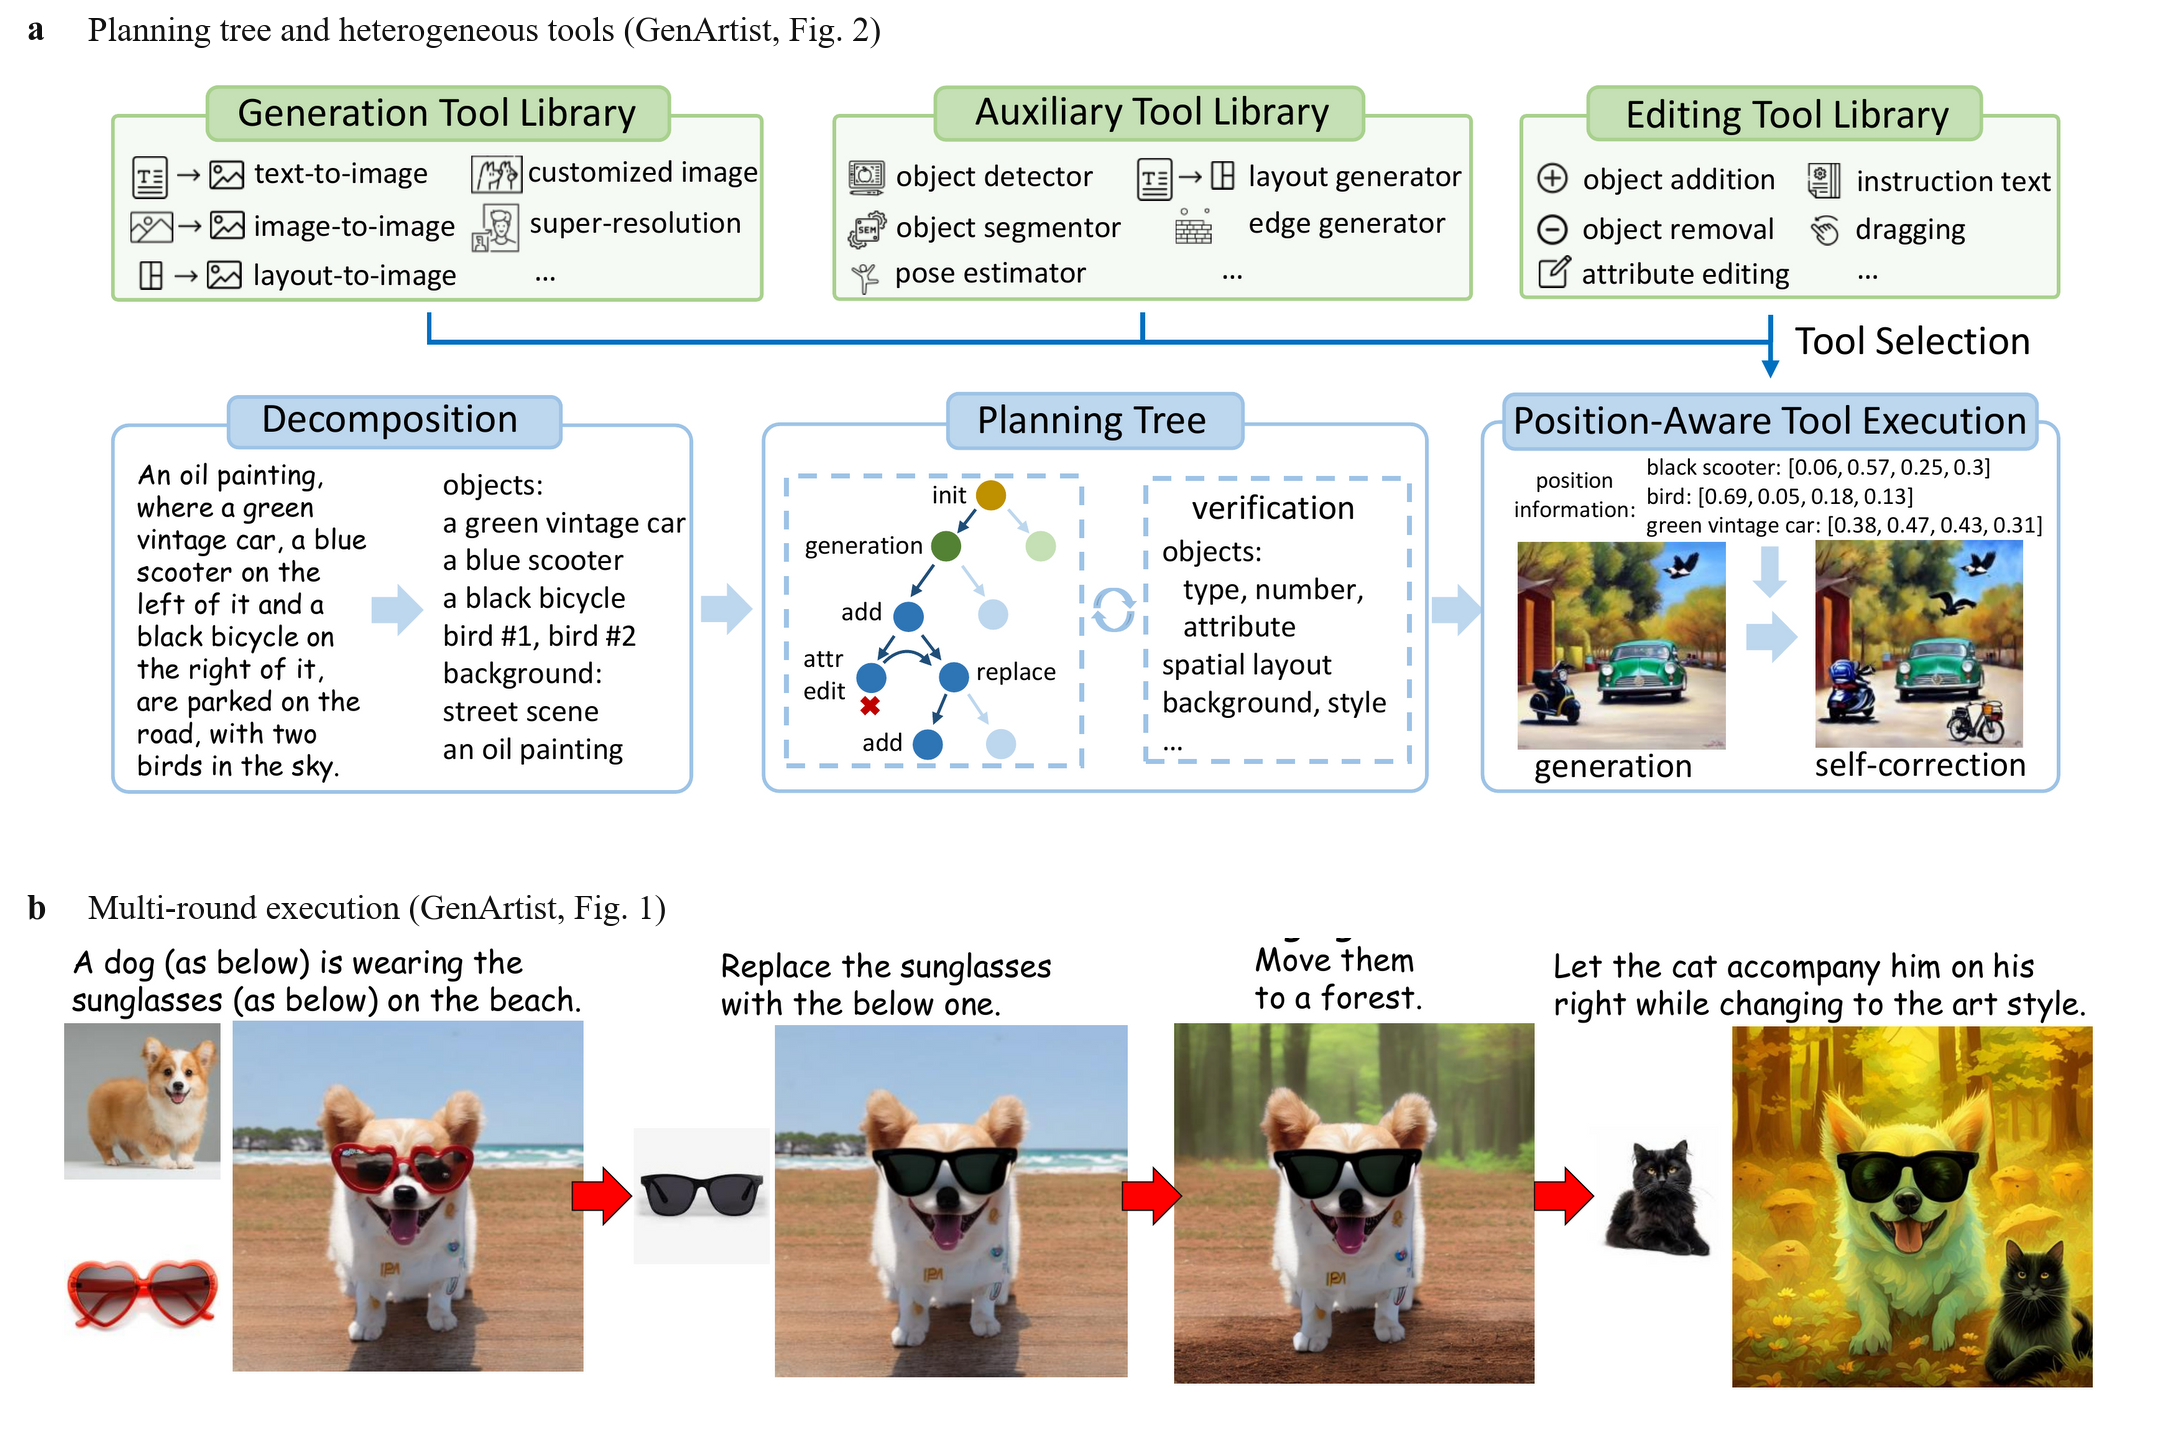
\includegraphics[width=\textwidth]{figures/ch4_planning_tool_orchestration.jpg}
  \caption{Executable planning and tool orchestration. GenArtist decomposes a complex request into a verified planning tree over generation, auxiliary, and editing tools, then carries the resulting state through multi-round execution~\cite{wang2024genartist}.}
  \label{fig:ch4-planning-tools}
\end{figure}

\paragraph{RestoreAgent.}
 is an MLLM-driven agent that selects task order and models for mixed image degradations (denoising, deraining, dehazing, deblurring, JPEG removal, low-light enhancement). A vision encoder + Llama3 controller predicts the next tool from current image and history, with step-wise reassessment and rollback on failure. ~\cite{avg240718035}

\paragraph{AgenticIR.}
 is an LLM/VLM-driven system that restores images with multiple interacting degradations (noise, blur, compression...) by composing specialist models via a perception–scheduling–execution–reflection–rescheduling loop; failed operations trigger rollback and re-planning. A fine-tuned DepictQA provides degradation descriptions and success judgments; offline exploration enumerates tool sequences on held-out images and summarizes success patterns into retrievable documents for scheduling.~\cite{avg241017809} Figure~\ref{fig:ch4-recovery} illustrates this artifact-conditioned reflection, rollback, and rescheduling loop.

\begin{figure}[!htbp]
  \centering
  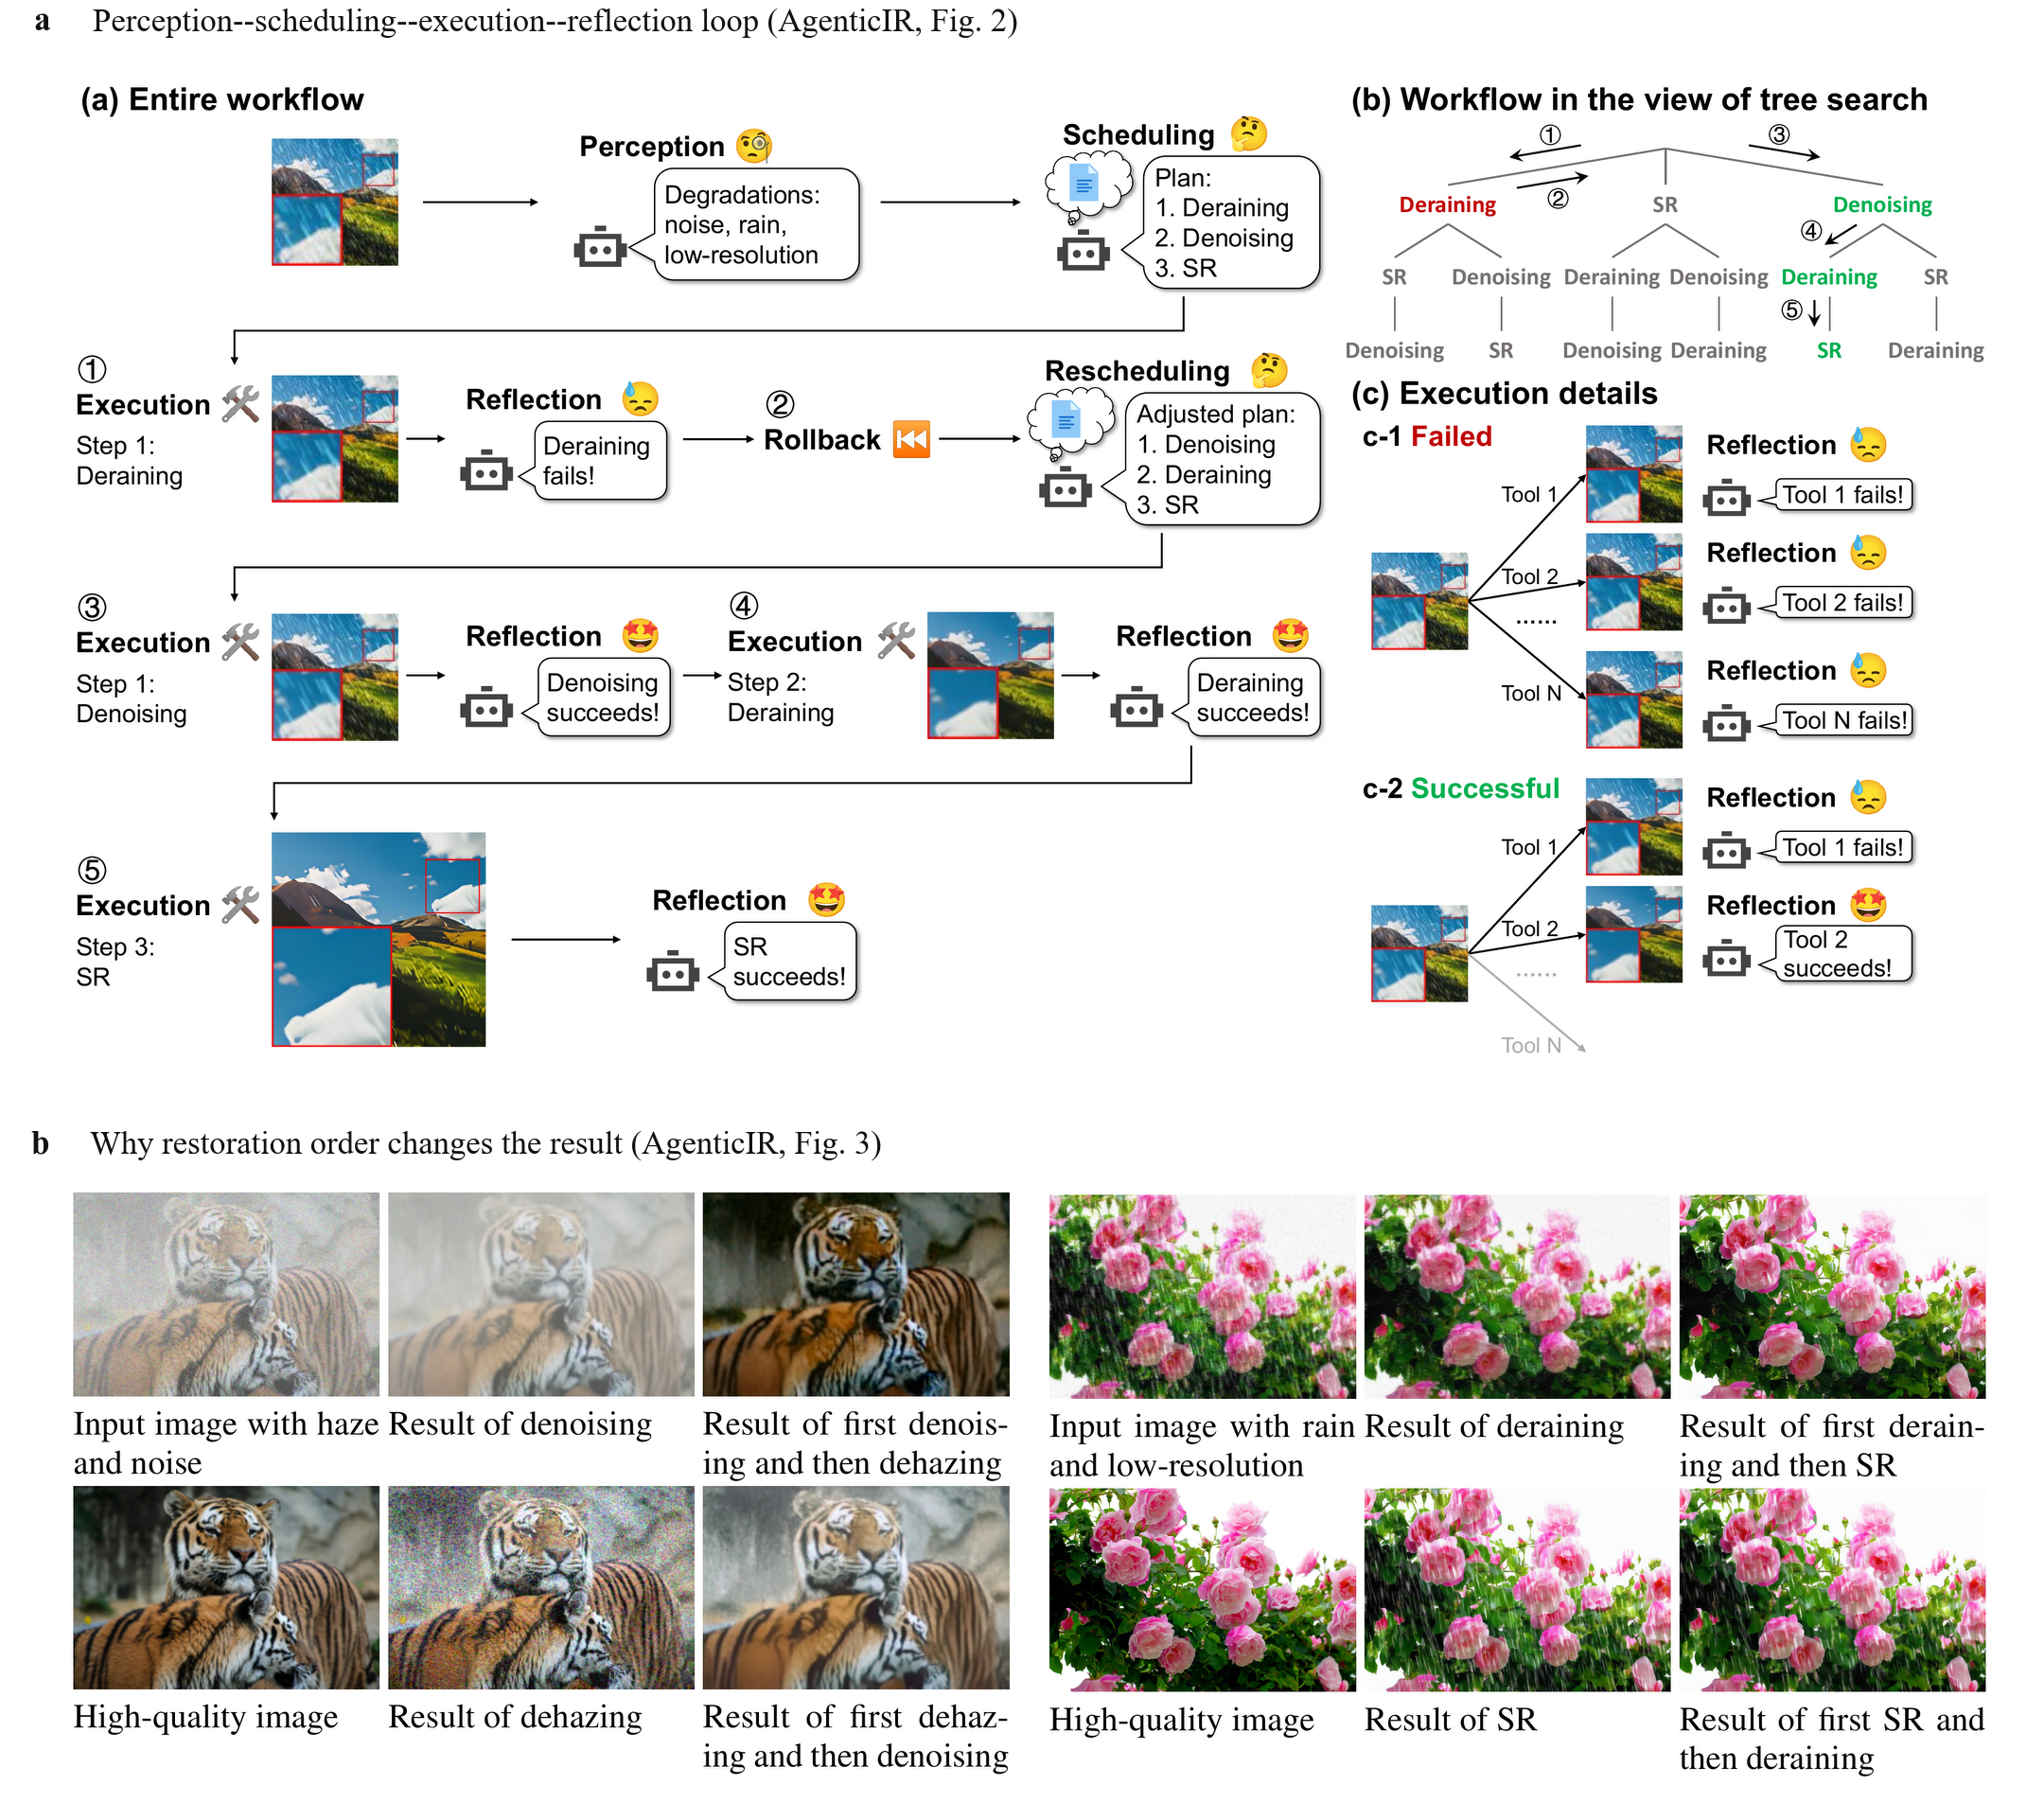
\includegraphics[width=\textwidth]{figures/ch4_reflection_recovery.jpg}
  \caption{Artifact-conditioned recovery in image restoration. AgenticIR observes degradation and execution outcomes, reflects on failed operations, rolls back, and reschedules the remaining tool sequence; the qualitative examples show why operation order changes restoration quality~\cite{avg241017809}.}
  \label{fig:ch4-recovery}
\end{figure}

\paragraph{HybridAgent.}
 is an agentic image restoration system with a FastAgent for direct prompts (routing tools in ~12\% of SlowAgent time) and a fine-tuned SlowAgent for ambiguous requests; a FeedbackAgent judges cleanness and can trigger further restoration. Tools are built via three-stage training (base model → LoRA single-task tools → mixed-degradation tool), enabling joint restoration to replace damaging long chains.~\cite{avg250310120}

\paragraph{CoSTA*.}
 is a cost-sensitive agent that plans and executes multi-turn image edits via LLM-driven subtask tree generation, tool subgraph construction over 24 tools, and A* search balancing quality and runtime with a tunable cost-quality parameter; a VLM validator checks each subtask and triggers retries or alternative paths on failure. ~\cite{gupta2025costa}

\paragraph{ComfyGPT}
 is a multi-agent system that generates executable ComfyUI workflows from natural-language task descriptions. ReformatAgent converts JSON workflows to link-centered diagrams, FlowAgent predicts diagrams (trained with SFT + GRPO with validity rewards), RefineAgent retrieves current node definitions from a database to replace invalid nodes, and ExecuteAgent submits the final workflow. ~\cite{huang2025comfygpt}

\paragraph{Q-Agent.}
 is a quality-driven image restoration (IR) agent that addresses multiple degradations via CoT-based perception and greedy IQA-guided restoration. A fine-tuned MLLM answers per-degradation Yes/No questions; at each step, all candidate operations are applied, ranked by an aggregate of five NR-IQA metrics, and the best is greedily selected until no improvement. ~\cite{avg250407148}

\paragraph{FaSTA*.}
 extends CoSTA* by mining reusable tool sequences (subroutines) from prior traces via LLM-based inductive reasoning and storing them with activation conditions in a rule table. It first attempts fast planning using these rules, with VLM checks validating each subroutine; only when no rule applies or a check fails does it fall back to localized A* search. ~\cite{gupta2025fasta}

\paragraph{Restore-R1.}
 is a lightweight reinforcement-learned agent that predicts restoration tool sequences in a single forward pass, eliminating runtime reflection/rollback. A CLIP+MLP policy is trained via PPO/GRPO using DeQA-Score as the reward, without ground-truth labels. ~\cite{avg251218599}

\paragraph{Derain-Agent.}
 is a plug-and-play post-deraining enhancer that refines initial derained outputs by predicting one of 16 predefined tool paths (denoising, deblurring, color correction) and pixel-wise strength maps from a ResNet34 feature extractor, then executing the path once. ~\cite{avg260311866}

\paragraph{TIR-Agent.}
is a trainable VLM agent that learns direct tool-calling policies for multi-degradation restoration via SFT + RL, replacing costly heuristic search. A Qwen3-VL-8B controller selects task and model per step from current image and history; EDP diversifies SFT trajectories, while MAR dynamically reweights FR/NR metrics to prevent reward hacking. ~\cite{avg260327742}

\paragraph{IMAGAgent.}
 is a plan–execute–reflect agent for multi-turn image editing that prevents error accumulation and semantic drift. A VLM planner decomposes instructions into atomic sub-tasks; a controller dynamically composes segmentation, detection, retrieval, and editing tools from the current image and history; multiple VLM experts critique intermediate outputs; and an aggregator converts feedback into corrective actions, with up to three retries per turn. ~\cite{avg260329602}

\paragraph{Adaptive Task Reformulation.}
ATR improves image editing by reformulating ambiguous tasks without modifying the backbone. A profiler extracts target and scene context; a router selects direct/rewritten editing, spatial decoupling, or localized workspace; a planner executes sequentially with state, feedback, and fallback. ~\cite{avg260415917}

\paragraph{From Plans to Pixels.}
 is an experiential learning framework for long-horizon advertisement editing. A checklist-guided planner decomposes abstract instructions into subtasks; a reward-trained orchestrator selects tools/regions from a heterogeneous editor library; a VLM judge provides outcome rewards, infeasible subtasks are pruned, and a distilled verifier re-ranks intermediate candidates. ~\cite{avg260515181}

\paragraph{OPERA}
 is an end-to-end framework for multi-tool cooperative image restoration. A GRPO-trained planning agent emits complete tool compositions directly from the input, receiving final restoration quality as reward; 16 restoration tools are jointly fine-tuned through generated chains, enabling cooperative behavior. ~\cite{avg260522104}

\paragraph{GenClaw.}
 is a code-driven agentic image generation framework that decouples creation into Conceptualize–Sketch–Color stages: it retrieves contextual knowledge via search/reasoning, constructs executable visual code (SVG/HTML/Canvas/Three.js) as an intermediate layout, then renders photorealism via an image generator. ~\cite{ye2026genclaw}

\paragraph{DiTTo.}
 is an order-aware restoration agent framework that decouples training from real-expert calls via a simulator (US-IR + AiO-IQA) that reduces ORTD construction from $\mathcal{O}((N^{\mathrm{D}})^2)$ to $\mathcal{O}(N^{\mathrm{D}})$ calls. A VLM agent is SFT-trained on simulated trajectories, then aligned to a small real-expert set via decomposed DPO (DP/OR/Tool axes); new experts require updating only the alignment stage.~\cite{avg260530915}

\paragraph{IEA.}
 is an amateur-friendly conversational editor that performs global photo retouching via 16 parameterized tools (brightness, exposure, contrast, etc.), emitting explicit tool calls rather than synthesizing pixels. A Qwen2.5-VL-7B policy is trained in three stages: Stage 1 distills expert programs from GIER for SFT; Stage 2 applies GRPO with likeness and usefulness rewards; Stage 3 adds synthetic Image-Edit, Image-Summary, and Image-Refine data to enable history summarization and feedback-driven refinement. ~\cite{avg260608016}

\paragraph{CanvasAgent.}
 is a tool-augmented agent for complex multi-step image workflows across 11 tools (generation, edit, grounding, etc.). Trained via SFT + GRPO on CanvasCraft (140K SFT trajectories + 10K RL tasks), it maintains asset state, supports plan revision and rollback. SFT+RL substantially outperforms SFT-only across overall reward, alignment, and trajectory quality; human evaluation also favors it over Qwen3-VL-32B.~\cite{avg260705465}


\subsection{Stateful Image Generation and Editing}
Stateful image systems retain information needed to preserve identity, user intent, scene structure, and earlier decisions. The literature separates turn-level user and context management from explicit scene, narrative, and trajectory representations.

\subsubsection{Multi-Turn User, Subject, and Context Management}
These systems retain information that is needed across turns, including user preferences, subject identity, prior operations, context, and candidate quality. The persistent representation makes a later action dependent on more than the current prompt.

\paragraph{AutoStudio.}
 is a training-free multi-agent framework for multi-turn interactive image generation. It stores subject features with persistent IDs; a subject manager parses dialogue, a layout generator predicts bounding boxes, a supervisor refines spatial relations, and a P-UNet drawer renders the final image via subject-initialized generation.~\cite{cheng2024autostudio}

\paragraph{Preference Adaptive and Sequential Text-to-Image Generation (PASTA)}
 is an RL agent for multi-turn T2I generation that iteratively refines prompts via adaptive expansion slates guided by user selections and a learned preference model. Trained on 7,000 human rater sequences + 30,000 simulated rollouts, its user model achieves ~70\% accuracy on held-out metrics.  ~\cite{nabati2025pasta}

\paragraph{StoryState.}
 is an agent-based state controller for consistent and editable storybooks. It externalizes each story as $S=(C,W,\{S_i\})$—a character sheet, global world state, and page-level scene states—maintained by Planner and State Manager agents. A Prompt Writer maps this state to global/page prompts; local edits update a single $S_i$, identity edits update $C$ and propagate to affected pages; a Consistency Critic verifies outputs against the state and neighboring pages. ~\cite{sarkar2026storystate}

\paragraph{Agent Banana.}
 is a hierarchical planner-executor agentic framework for professional image editing that addresses over-editing, multi-turn fidelity loss, and native 4K resolution. It decomposes vague instructions into atomic operations, performs localized editing via Image Layer Decomposition to preserve non-target regions, and uses Context Folding for stable long-horizon state tracking, with self-reflection enabling retry, rollback, and replanning. ~\cite{ye2026agentbanana}. 

\paragraph{Generation Navigator.}
 frames multi-turn text-to-image generation as a state-conditioned action-making problem, where a learned multimodal navigator dynamically chooses to STOP, REFINE, or REGENERATE based on the current image and reviewer feedback~\cite{avg260517969}. To train this policy, the system constructs 103K trajectories and applies PRE-GRPO, a trajectory-level reinforcement learning objective that jointly rewards peak quality, retention against degradation, and turn efficiency. 

\subsubsection{Scene, Narrative, and Trajectory State Management}
For multi-object edits and visual narratives, systems externalize scene structure, causal relations, candidate branches, or operation histories. This turns an image sequence into an addressable state space for planning and recovery.

\paragraph{I2E}
 reformulates compositional image editing as interaction within a structured environment, using a Decomposer to segment objects, recover occlusions, and build physically ordered layers via DAG-based spatial propagation~\cite{avg260103741}. A physics-aware VLA Editor translates instructions into atomic actions (REMOVE, MOVE, FALL, RESIZE, EDIT, INSERT) through chain-of-thought reasoning, executing object-level edits without global pixel resampling.

\paragraph{MSRAMIE}
 is a training-free multimodal agent framework that handles complex multi-instruction image editing by decomposing lengthy requests into structured sub-tasks through iterative interactions between an MLLM-based Instructor and a plug-in editing Actor~\cite{avg260316967}. It constructs a Tree-of-States for flexible state transitions, backtracking, and resampling, while a Graph-of-References retrieves nearby states to avoid redundant exploration. 

\paragraph{LogiStory.}
 targets multi-image story visualization by explicitly modeling visual logic—causal and perceptual coherence across characters, actions, and scenes over time~\cite{avg260328082}. A multi-agent system extracts entities, causal events, and panel scripts; a Local Causal Monitor checks each frame against accumulated narrative memory, while a Global Causal Verifier maintains a story-level causal graph and triggers regeneration or editing upon inconsistency.

\subsection{Multi-Agent Systems for Image Generation and Editing}
Multi-agent systems allocate visual creation work among specialized roles. Their value depends on how role outputs, shared state, and evaluator feedback determine later actions, rather than on the number of participating agents.

\subsubsection{Collaborative Generation, Composition, and Domain Design}
This group distributes generation, analysis, design, or evaluation work across specialized roles. It includes contextual comparisons that clarify the difference between model-level cooperation and task-level visual creation control.

\paragraph{Message Passing Multi-Agent GANs.}
This early work explores unsupervised image generation with two generators that share a discriminator and exchange learned messages via a common message generator, with competing or conceding objectives encouraging complementary behavior~\cite{avg161201294}. 

\paragraph{Anywhere.}
 replaces end-to-end inpainting with a multi-agent pipeline for foreground-conditioned image generation, preserving object integrity and supporting optional text guidance~\cite{xie2024anywhere}. A Foreground Analyzer and Prompt Creator generate scene prompts; a Template Repainter repairs mask violations; and a Quality Evaluator triggers regeneration when needed.

\paragraph{Marmot.}
 addresses counting, attribute-binding, and spatial errors in text-to-image generation via object-level divide-and-conquer~\cite{sun2025marmot}. An Object-Aware Agent decomposes the scene into subtasks; an Object Correction System with decision-execution-verification operates on individual masks or object-pair boxes, retrying upon failure; a Pixel-Domain Stitching Smoother merges corrected regions via mask-guided optimization.

\paragraph{MCCD}
 enhances complex text-to-image generation through a multi-agent parsing module and hierarchical compositional diffusion~\cite{avg250502648}. A conductor schedules six specialist agents with forward reasoning and evaluator-triggered backward feedback; the diffusion module renders parsed elements via depth-aware Gaussian masks, regional enhancement, and boundary smoothing.

\paragraph{T2I-Copilot.}
 addresses ambiguous text-to-image prompts through a training-free multi-agent system that interprets user intent, selects appropriate models, and iteratively refines outputs~\cite{chen2025t2icopilot}. An Input Interpreter extracts entities, attributes, and ambiguities; a Generation Engine selects and executes the optimal generation or editing route; and a Quality Evaluator scores aesthetic and alignment criteria, triggering regeneration with structured suggestions when scores fall below a threshold. 

\paragraph{From Image Generation to Infrastructure Design.}
This work applies multi-agent image editing to bicycle-lane visualization as a constrained street-scene editing problem~\cite{avg250905469}. A Locator Agent identifies roadway geometry; a Prompt Agent formalizes user intent; a Design Generation Agent produces candidates via highlight-first cascading; and an Evaluator Agent reranks candidates and verifies hard constraints, triggering regeneration when none pass.

\paragraph{GenPilot.}
 optimizes text-to-image prompts at test- time via a multi-agent system that iteratively refines inputs to improve semantic alignment~\cite{avg251007217}. An error-analysis stage decomposes prompts and combines VQA with caption comparison to localize mismatches; a test-time optimization stage generates candidate rewrites, scores them with an MLLM, clusters candidates, and uses memory to guide subsequent rounds.

\paragraph{Collaborative Text-to-Image Generation.}
This work explores multimodal text-to-image generation via domain-specialized agents (architecture, portraiture, landscape) coupled with PPO training and multimodal fusion~\cite{avg251010633}. A text-enhancement subsystem and an image-generation subsystem each contain specialized agents; PPO optimizes them with a composite reward over similarity, quality, and diversity, while contrastive learning and bidirectional attention enforce cross-modal alignment. 


\paragraph{M3.}
 is a training-free multi-agent framework that refines text-to-image outputs through iterative, validated editing~\cite{avg260206166}. A Planner decomposes prompts into checklists; a Checker evaluates each constraint; a Refiner generates edit instructions for failures; an Editor executes edits; and a Verifier accepts only edits that improve alignment over the previous best. 

\paragraph{coDrawAgents.}
 is a multi-agent  framework for compositional text-to-image generation where an Interpreter adaptively chooses between direct generation and layout-aware mode~\cite{avg260312829}. In layout-aware mode, a Planner incrementally proposes placements for priority-grouped objects grounded in the evolving canvas, a Checker validates and refines spatial and semantic consistency, and a Painter synthesizes the partial image to inform subsequent iterations. 


\paragraph{InterleaveThinker.}
 enables long-horizon interleaved text-image generation by decoupling global planning from stepwise execution through a multi-agent framework~\cite{avg260613679}. A Planner produces an N-step plan upfront; at each step, a frozen image generator executes the instruction, and a Critic evaluates the result against the plan, issuing binary judgments and refined prompts. The Critic is trained with dual-reward GRPO combining judgment accuracy and correction quality. 

\paragraph{AuDiffusion.}
 is a multi-agent diffusion framework with Prompt, Layout, and Executor agents for controllable text-to-image generation~\cite{avgdoi101007s40747025022111}. The Prompt Agent enriches semantics; the Layout Agent selects ControlNet modules via capability-requirement matching; the Executor synthesizes images using an AuMamba backbone with linear-time state-space scans and windowed attention. A shared blackboard stores states and triggers targeted revisions when quality falls below threshold.

\paragraph{Multi-agent Collaborative Pathways for Chinese Traditional Architectural Image Generation.}
\textbf{Problem and setting.} This system generates images of Chinese traditional architecture from non-specialist requests while attempting to preserve historically specific form, color systems, decorative symbols, and cultural meaning~\cite{avgdoi101038s41598025181307}. \textbf{Method and mechanism.} A domain knowledge base encodes entities, architectural components, spatial rules, symbolism, and historical versions. Intent understanding and prompt-generation agents ground vague requests in this knowledge; a Stable Diffusion LoRA plus Canny ControlNet renders the image. An aesthetic and cultural-relevance agent returns scores and error flags to a workflow scheduler. Depending on the diagnosed cause, the scheduler revisits prompt generation, changes rendering parameters, or returns to intent interpretation, with a maximum iteration count preventing unbounded execution. \textbf{Evaluation and results.} Sixty participants, comprising 20 domain experts, 20 relevant students, and 20 general users, score anonymized outputs. The MAS prototype reports $4.65\pm0.25$ for architectural form, $4.72\pm0.20$ for color fidelity, and $4.71\pm0.22$ for decorative-symbol consistency, compared with $4.50\pm0.28$, $4.58\pm0.26$, and $4.61\pm0.29$ for the same generator driven by expert-authored prompts. Its average CLIP score is $0.89\pm0.03$, compared with $0.86\pm0.04$ for that baseline. \textbf{Evidence boundary.} Visual and cultural error reports determine targeted rerouting, providing L3 artifact-conditioned correction. The evidence comes from one cultural case study and an author-built knowledge base; CLIP against the optimized prompt is not a direct measure of historical truth, and the evaluation does not isolate the contribution of repeated correction from knowledge grounding and model specialization. A single pass averages about 166.7 seconds, with additional iteration cost.

\paragraph{MUSES}
 generates 2D images with precise 3D control by leveraging 3D layouts, models, and rendering as intermediate guidance~\cite{ding2025muses}. A Layout Manager plans 2D layouts via in-context learning and lifts them to 3D (depth, orientation, camera) via chain-of-thought; a Model Engineer retrieves or generates 3D assets and aligns them to camera using a fine-tuned CLIP classifier; an Image Artist assembles the scene in Blender and renders depth/Canny controls for final diffusion. Figure~\ref{fig:ch4-structured-control} shows how typed 2D and 3D intermediates coordinate these specialized agents.

\begin{figure}[!htbp]
  \centering
  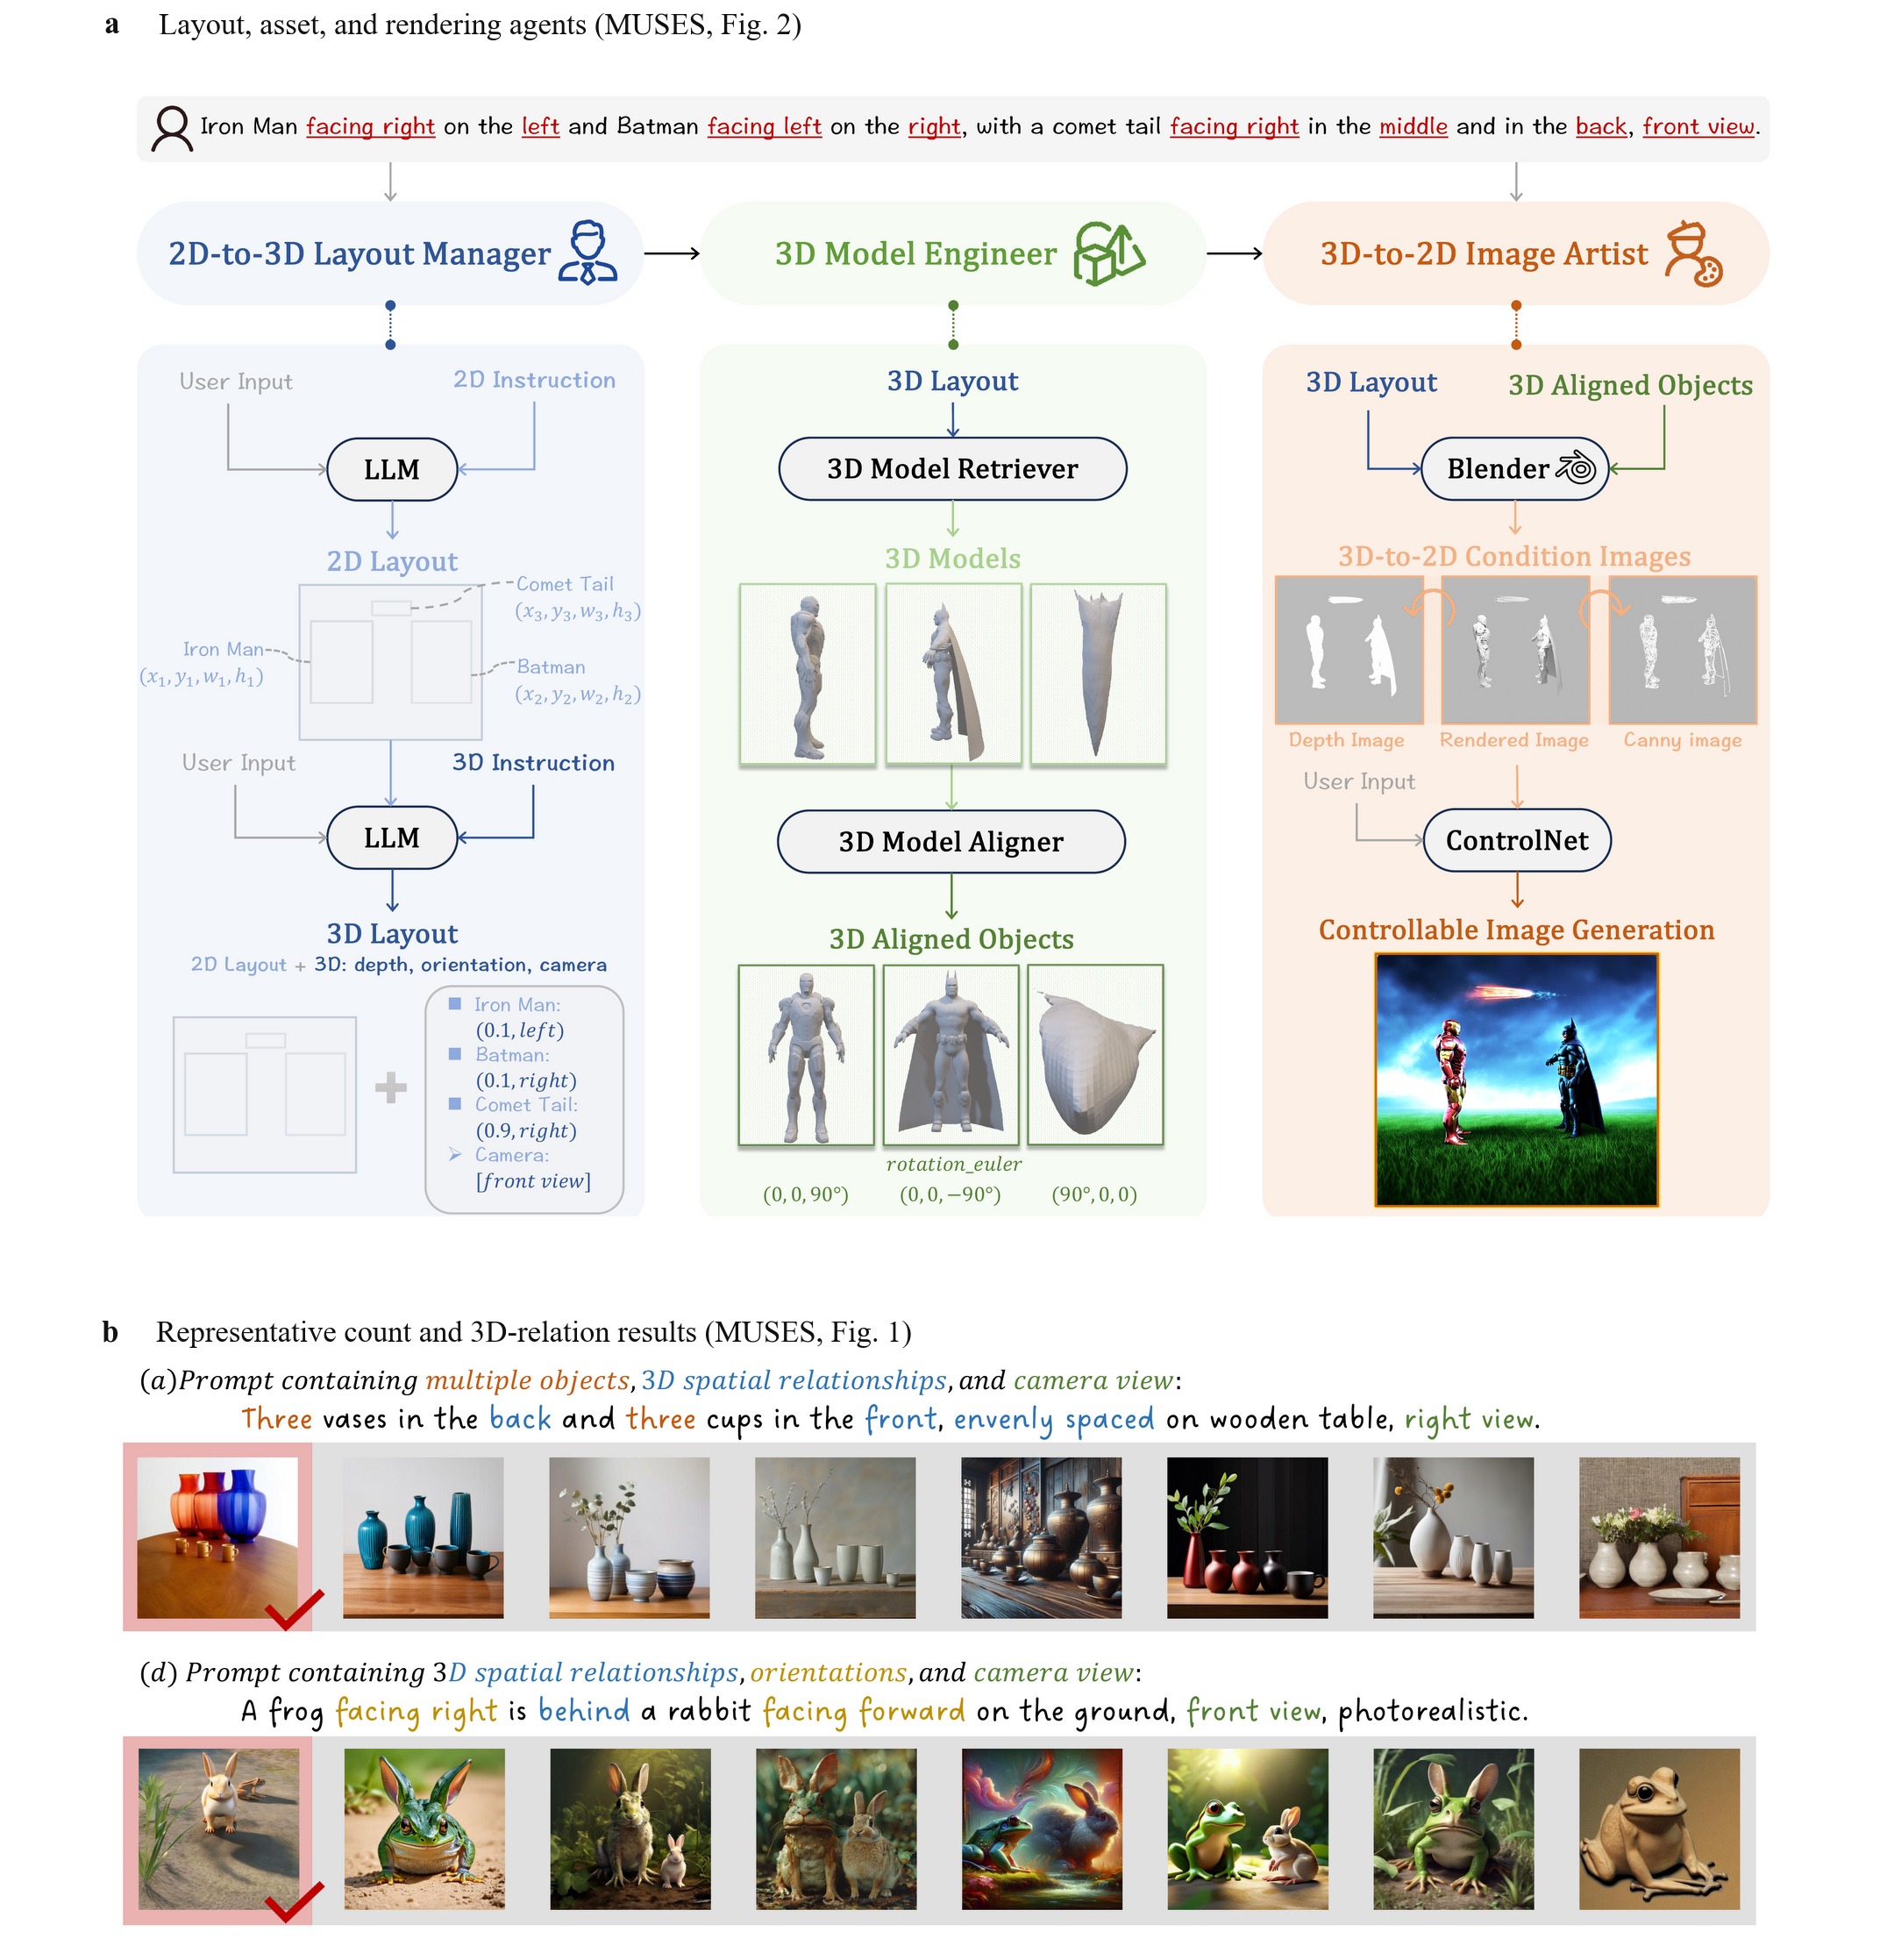
\includegraphics[width=\textwidth]{figures/ch4_multi_agent_structured_control.jpg}
  \caption{Structured multi-agent control through typed intermediate representations. MUSES converts language into 2D and 3D layouts, aligned assets, rendered control signals, and a final image; representative comparisons illustrate count and 3D-relation constraints~\cite{ding2025muses}.}
  \label{fig:ch4-structured-control}
\end{figure}


\subsubsection{Collaborative Editing, Completion, and Restoration}
These systems divide image modification into complementary planning, execution, evaluation, and specialized restoration or completion roles. Their evidence concerns whether this division improves an evolving edited artifact.

\paragraph{CCA}
 addresses complex image editing by deploying two generator agents that independently decompose instructions and execute tools, and a discriminator that compares outputs, provides subtask-level feedback, and triggers parameter adjustments or tool reselection across rounds~\cite{hang2024cca}. A best-candidate bank enables cross-round comparison, with early stopping when quality meets requirements (up to five rounds). 

\paragraph{MAIR}
 is a multi-agent system for complex image restoration, guided by a real-world degradation prior that reverses scene, imaging, and compression artifacts in sequence~\cite{avg250309403}. A Scheduler agent plans the overall restoration order using perception, textual experience, and user instructions; Expert agents then sequentially remove specific degradations by selecting from registered tools, executing, and reflecting on results before passing to the next. 

\paragraph{CREA}
 is a multi-agent framework for creative image editing and generation~\cite{venkatesh2025crea}. A Creative Director sets the vision; a Prompt Architect fuses six creativity-principled prompts; a Generative Executor synthesizes images; a Critic scores six creative dimensions; and a Refinement Strategist adjusts prompts over up to three iterative rounds based on weak scores.

\paragraph{Talk2Image.}
 is a multi-agent system for multi-turn conversational image generation and editing, where later instructions accumulate with earlier scene content and affect only requested regions~\cite{avg250806916}. A multi-turn intention parser converts dialogue history into structured cumulative specifications; specialized agents execute generation, editing, segmentation, VQA, and chat via DAG-scheduled operations with blackboard-based coordination; and multi-view feedback scores semantic alignment and visual consistency, triggering retries until a threshold is met. 

\paragraph{Multi-Agent Amodal Completion.}
This multi-agent framework reconstructs occluded or truncated objects and outputs layered RGBA assets~\cite{avg250917757}. An Occlusion Agent identifies front-back relations, a Segmentation Agent extracts masks, a Boundary Agent estimates canvas expansion, and a Description Agent provides semantic guidance; these upfront decisions define a single inpainting mask and prompt for one-pass FLUX-ControlNet synthesis, with attention maps fused to generate the alpha channel.

\paragraph{ImageEdit-R1.}
 addresses complex, multi-step image editing instructions through a reinforcement learning-enhanced multi-agent framework~\cite{avg260308059}. A decomposition agent (Qwen2.5-VL-7B) parses user requests into actions, subjects, and goals; a sequencing agent orders sub-requests; a diffusion-based editor executes them. GRPO trains the decomposition agent with format, action, subject, and goal rewards without modifying the editor.

\paragraph{CAMEO}
 is a hierarchical multi-agent framework for conditional image editing that replaces single-pass generation with quality-aware, feedback-driven refinement~\cite{pu2026cameo}. A Strategic Director interprets requests and selects constraints; a Visual Research Specialist retrieves or synthesizes references; a Quality Critic evaluates intermediate outputs across task-adaptive dimensions and returns structured deviations; and a Refinement Editor applies targeted corrections, looping until thresholds are met. 

\paragraph{APE}
 is a lightweight framework that post-trains small language models as prompt enhancers for image generation and editing  without modifying downstream models~\cite{avg260600204}. Its single-agent (SAPE) and multi-agent (MAPE) variants decompose enhancement into router-selected field rewriting and composer fusion, trained via SFT and GRPO/GDPO on downstream rewards (PickScore, CLIPScore, HPSv2.1, GPT-based editing judgments). 


\subsection{Native and Unified Agentic Models for Image Creation}
Native and unified models place reasoning, understanding, generation, and sometimes tool use within a common multimodal policy. This organization is discussed separately from the feedback and workflow mechanisms analyzed in earlier groups.

\subsubsection{Native and Unified Models for Reasoning and Generation}
Native and unified models integrate image understanding, reasoning, and generation in one learned policy. The grouping concerns the implementation locus of these functions, not an automatic claim of high autonomy.

\paragraph{ImAgent.}
 is a training-free unified multimodal agent that enables adaptive test-time scaling for image generation and editing through a policy controller that dynamically selects actions based on observation history~\cite{avg251111483}. Built on a single UMM, its action space includes direct generation/editing, CoT prompt enhancement, image-conditioned prompt revision, local detail refinement, Best-of-N sampling, and STOP; invalid actions fall back to direct generation. 

\paragraph{UniReason 1.0.}
 unifies text-to-image generation and editing within a shared framework for requests requiring implicit world knowledge~\cite{avg260202437}. World-knowledge-enhanced textual reasoning expands underspecified prompts into explicit guidance before synthesis; the model then observes the generated image, reflects, and applies editing-style refinement to correct discrepancies. Training uses an agent pipeline (generator → verifier → refiner → judge) and two-stage SFT on reasoning and interleaved refinement samples.

\paragraph{VisionCreator.}
 is a native visual-generation agentic model unifying Understanding, Thinking, Planning, and Creation for complex image/video creation with multi-step tool invocation~\cite{avg260302681}. Progressive Specialization Training uses 4k expert-filtered trajectories, while Virtual Reinforcement Learning optimizes long-horizon planning in a simulated 36-tool environment with plan, format, execution, result, consistency, and trajectory rewards; average trajectories span 15 steps (64\% >20).



\paragraph{VisionCreator-R1.}
 extends VisionCreator's UTPC framework with Reflection, forming a UTPCR loop that inspects intermediate images, identifies deviations, and triggers targeted edits or regeneration~\cite{avg260308812}. Reflection-Plan Co-Optimization first learns reflection on single-image tasks, then mixes reflection-strong and planning-strong trajectories before multi-task RL with reflection, plan, format, tool, and result rewards.


\subsubsection{Models for Grounded, Spatial, and Open-World Creation}
This group extends unified policies to world knowledge, spatial reasoning, and tool-mediated open-world generation. It concentrates on models whose primary contribution is grounded creation within an integrated multimodal policy.

\paragraph{Unify-Agent.}
 is an end-to-end unified multimodal agent for world-grounded image synthesis, reformulating generation as a sequential process of prompt understanding, multimodal evidence search, grounded recaptioning, and final synthesis~\cite{avg260329620}.  A unified model diagnoses missing knowledge, performs textual and visual search, and transforms retrieved evidence into a compact recaption trained on 143k annotated trajectories.

\paragraph{Boogu-Image-0.1.}
 is an open image-generation and editing model family designed for complex, multilingual, and text-rich requirements under constrained budgets~\cite{avg260713125}. Its core generator uses Qwen3-VL-8B as instruction encoder with a curated data syllabus; at inference, a DeepSeek-V4-Flash agent performs reasoning-oriented prompt rewriting and routes between Base and Turbo variants by task complexity, with reflection and Best-of-N as optional scaling. 

\paragraph{ToolArtist.}
 is a fully agentic image-generation model obtained by post-training a unified multimodal model, where reasoning, external tool use, and native image generation are coordinated within a single policy~\cite{zhao2026toolartist}. Supervised trajectories are collected from a teacher agent with search and generation tools then converted to UMM-native format; RAD-GRPO jointly optimizes with intent and quality rewards. 

\subsection{Data, Evaluation, and Safety for Agentic Image Generation}
Data construction, learning, evaluation, and safety research supports the development and assessment of image agents. These studies determine how controllers are trained, what claims of reusable experience are supported, and how quality or safety failures can be measured.

\subsubsection{Data Construction, Policy Learning, and Reusable Experience}
This group studies how visual-agent data, policies, workflows, and experience stores are constructed or improved. The central question is what, if anything, persists beyond a single trajectory and improves a later task.

\paragraph{Gen-n-Val.}
 is an agentic framework for generating synthetic instance segmentation data to address data scarcity and long-tailed imbalance~\cite{huang2025gennval}. A TextGrad-optimized LLM generates detailed prompts for Layer Diffusion to produce transparent single-instance foregrounds with alpha-channel masks; a VLM validator checks class identity, single view, object integrity, and plain background before accepted instances are composited into training scenes. 

\paragraph{SIDiffAgent.}
 is a training-free self-improving diffusion agent that refines text-to-image generation via iterative prompt engineering, evaluation, and editing, supported by experience memory~\cite{avg260202051}. An orchestrator handles intent analysis and adaptive negative prompting; an evaluator triggers up to two corrections; a guidance agent stores and retrieves past trajectories to guide future generations.



\paragraph{Socratic-Geo.}
 is an autonomous multi-agent framework for geometry data synthesis and reasoning, where a Solver's failed attempts trigger a Teacher to diagnose gaps, modify parameterized Python drawing code, and validate new problems via Reflect (solvability) and RePI (visual validity) before adding them to the curriculum~\cite{avg260203414}. A Generator is separately fine-tuned on accumulated image-code-instruction triplets to distill programmatic drawing into diffusion-based generation. 

\paragraph{PaAgent.}
  is a portrait-aware image restoration agent that selects restoration experts via a self-evolving portrait bank with RAG, while subjective-objective RL with GRPO refines its degradation perception.~\cite{avg260317055}. A Qwen-based module perceives degradation using images, scores, and task history; RAG queries a bank of stored triplets to recommend the next expert, with each interaction added back to the bank.



\paragraph{ScaleEdit-12M}
 ScaleEditor is an open-source multi-agent framework for constructing large-scale image editing datasets without costly commercial APIs, producing 12M instruction-image-edit triplets across 23 tasks~\cite{avg260320644}. Source image expansion combines retrieval and synthesis; a task router assigns images to specialized editing agents; task-aware verification scores instruction following, editing consistency, and generation quality, retaining only high-scoring pairs. 



\paragraph{GenEvolve.}
 is a self-evolving framework for open-ended image generation where an orchestrates factual search, visual reference retrieval, internal generation knowledge, and prompt-reference program synthesis along tool-based trajectories~\cite{chen2026genevolve}. It uses SFT cold-start, GRPO for trajectory-level optimization, and Tool-Orchestrated Visual Experience Distillation: comparing best-worst trajectories, extracting structured experience slots, conditioning a privileged teacher on retrieved experience, and distilling token-level preferences into the student policy.


\paragraph{EvoIR-Agent.}
 is a self-evolving image restoration agent that reduces trial-and-error in selecting restoration order and tools by reusing experience ~\cite{avg260522208}. A hierarchical experience pool stores guidance at three granularities: high-level insights, degradation-type mappings, and fine-grained pattern records; after batch accumulation, an evolution procedure updates entries and stabilizes priorities from quality rankings via Bradley-Terry-Davidson modeling, enabling later retrieval of outcome-reflected guidance. 

\paragraph{OctoT2I.}
 is an agentic router that selects among T2I models to jointly optimize generation quality and inference efficiency, with a self-evolving knowledge base built without human supervision~\cite{jiang2026octot2i}. During inference, a stateful multi-round router consults long-term tool knowledge and task-local memory, selects a generator, evaluates alignment, and stores the score for subsequent decisions. A Propose–Solve–Evaluate–Learn loop defines conceptual dimensions, generates exploration prompts, measures each tool's Pass@1, prunes mastered combinations, and updates empirical and semantic profiles.

\paragraph{A Task-Driven and Quality-Assured Agent Framework for SAR Data Generation.}
SAGA is a schema-grounded agent framework for SAR data augmentation, conditioning generation decisions on dataset structure, task objectives, and verification evidence rather than fixed pipelines~\cite{avg260628896}. It profiles datasets into validated schemas, ranks plans via benefit-cost-risk scoring, compiles them into recipe DAGs, and evaluates outputs through observer checks with bounded repair; policy memory stores evidence for reuse.

\paragraph{Self-Evolving Agentic Image Restoration via Deliberate Planning and Intuitive Execution.}
SEAR is a dual-process self-evolving agent for image restoration with coupled degradations, where a Deliberate Planner uses LLM scheduling and P-MCTS to explore long-horizon paths with hybrid rewards and MLLM tournament verification, while high-reward trajectories are distilled into episodic memory indexed by degradation fingerprints~\cite{avg260628971}. An Intuitive Executor retrieves stored strategies for recurring patterns, avoiding repeated search. 

\paragraph{DataEvolver.}
 is a self-evolving multi-agent framework for text-rich image data construction, treating rejected samples as feedback for improving subsequent collection rounds rather than discarding them~\cite{avg260631537}. A Retriever gathers candidates; a Verifier filters by quality, OCR, semantics, and duplicates; a Critic summarizes rejection patterns into semantic feedback for updating retrieval queries and prompts; and a Generator fills under-covered regions.

\paragraph{COMFYCLAW.}
 is a self-evolving skill harness for image-generation workflows in ComfyUI, where agents must construct valid graphs, satisfy node/model constraints, and repair visual failures across recurring tasks without rediscovering fixes~\cite{avg260701709}. It exposes stage-gated tools for typed DAG editing and rollback; a region-level VLM verifier translates visual defects into repair suggestions; successful trajectories and errors are distilled into skills, validated on held-out tasks before library commitment. 

\paragraph{Search Beyond What Can Be Taught.}
This work uses external search to ground knowledge-intensive text-to-image generation, but finds that naive retrieval corrupts outputs by overriding known concepts or injecting noise~\cite{wang2026searchgen}. It therefore co-trains a reasoner with a Gate-Filter-Integrate protocol to decide when and what to retrieve, alongside online DPO that expands the generator's parametric knowledge and rejection-sampling fine-tuning that recalibrates the reasoner to search only for what remains outside. 



\subsubsection{Evaluation and Safety}
Evaluation and safety studies provide the measurements and adversarial evidence needed to assess image-agent behavior. They are not treated as image-creation controllers merely because they use planning, search, or multiple roles.

\paragraph{A Unified Agentic Framework for Evaluating Conditional Image Generation.}
This work proposes CIGEVAL, an agentic framework that evaluates conditional image generation by decomposing tasks into fine-grained sub-questions, autonomously selecting tools like Grounding, Difference, Highlight, and Scene Graph to inspect specific visual aspects, and producing explainable scores with rationales. ~\cite{avg250407046}.

\paragraph{EdiVal-Agent.}
is an object-centric framework that evaluates multi-turn image editing by decomposing images into object pools, tracking their evolution across turns, and computing instruction-following (via detectors and VLMs on guided crops), content consistency (via DINOv3 similarity of unchanged objects and backgrounds), and visual quality (via HPSv3). ~\cite{avg250913399}.

\paragraph{Blueprint-Bench.}
 evaluates spatial reasoning by tasking models with converting apartment photographs into 2D floor plans, scoring outputs on room connectivity and size ranking~\cite{avg250925229}. Most LLMs, image generators, and agents perform at or below random baseline; human performance remains substantially superior, and iterative agent refinement does not meaningfully help.

\paragraph{Value-Aligned Prompt Moderation.}
VALOR moderates unsafe text-to-image prompts via a zero-shot agent that layers lexical, semantic, and value-level detection with intention disambiguation, selectively rewriting harmful requests and optionally triggering style-guided regeneration when generated images remain unsafe~\cite{avg251111693}. 

\paragraph{OrchJail.}
 jailbreaks tool-calling text-to-image agents by exploiting orchestration-level vulnerabilities, where individually benign tool calls compose into policy-violating outcomes. It learns causal relationships between prompt phrasing and tool-execution patterns from successful jailbreak traces, guiding mutation and scoring to efficiently search for prompts that trigger unsafe multi-step behaviors. ~\cite{avg260507414}.

\paragraph{Whispers in the Noise.}
This work reveals that concept erasure in diffusion models only disrupts early text-to-semantics mapping while leaving later noise-driven dynamics intact. ConceptAgent exploits this by injecting surrogate-preserved geometry and color into intermediate denoising states, bypassing the erased text-conditioning path. Experiments show it reliably awakens erased concepts across multiple erasure methods and backbones, outperforming baselines without training or model access~\cite{avg260518150}.


\paragraph{RedEdit.}
 red-teams image safety classifiers by formulating photo-editing evasion as a combinatorial search over edit sequences. A VLM proposes candidate edits while MCTS plans promising paths and backtracks from ineffective ones, requiring both detector evasion and content preservation. Experiments reveals systemic vulnerabilities in current moderation systems~\cite{avg260606140}.

\paragraph{Does AI Understand Imaging?.}
ImagingBench evaluates multimodal agents on computational imaging tasks including reconstruction, sensing, optics, and calibration. Across 20 subtasks and three protocols, agentic systems consistently underperform specialized methods, especially on lensless imaging, event reconstruction, time-of-flight, and holography; planner guidance offers only modest gains, and visually plausible outputs often have poor reference-based fidelity~\cite{avg260707189}.

These studies broaden assessment beyond final appearance to object-level edit correctness, spatial reasoning, physical fidelity, safety moderation, and verifier robustness. Their diagnostic outputs become evidence for AVG only when a separate controller uses them to choose a corrective action.

Across image tasks, corrective precision depends on whether the system retains an addressable representation of the artifact and connects verification evidence to a later action. Masks, object tables, edit histories, preference records, degradation estimates, and executable workflows can support localized revision; undifferentiated scores often lead to global resampling. The evidence remains uneven for verifier calibration, causal diagnosis, rollback, budget-aware stopping, and persistent improvement beyond one task.

\FloatBarrier
